\documentclass[titlepage]{article}
\usepackage[colorlinks=true]{hyperref}
\usepackage{graphicx}
\usepackage{caption}
\usepackage{titlesec}
\usepackage{algpseudocode}
\usepackage{algorithm}
\usepackage{algpseudocode}
\usepackage{amsmath}
\usepackage{wrapfig}
\setcounter{secnumdepth}{5}
\setcounter{tocdepth}{5}

\titleformat{\paragraph}{\normalfont\Large\bfseries}{\theparagraph}{1em}{}
\titlespacing*{\paragraph}{0pt}{3.5ex plus 1ex minus .2ex}{2.3ex plus .2ex}

\begin{document}

%simple command to add a figure 
%\myfigure{address}{caption}{width}
\newcommand{\myfigure}[3]{
\begin{figure}[h!]
  \centering
  \includegraphics[width=#3\textwidth]{#1}
  \caption{#2}
\end{figure}
}

\title{\huge KUKA Youbot Autonomous Robot: Controls and Planning Technical Plan}
\author{Ze Che\\
 \and
Chenkai Shao\\
\and
Edward Aguilar\\
\and
Ivan Jimenez\\
\and
Abraham Marsen\\
\and
Myron Lee}
\large\date{January 30, 2014\endgraf\bigskip\hrule\bigskip
Georgia Institute of Technology (GT)\\
GT Vertically Integrated Projects (VIP)\\
Georgia Tech Research Institute (GTRI)\\
GTRI Robotics VIP Team
}
\maketitle
\tableofcontents
\section{Introduction}
In the field of agriculture, there is a constant issue of labor cost vs consumer prices. Because of the naturally erratic nature of plant-life, harvesting presents a particularly complex problem to both hardware and software and has thus been left to seasonal workers, which in both recent and coming years has driven the price of produce up as the wage of these workers has risen. With this in mind, it is imperative that a system to replace these costs step in to fill the gap in order to keep consumer prices down. Already, there are products out there that are in the early stages of this task, with examples such as the Intelligent Robotic Vineyard Pruner from Vision Robotics Corp. and Wall-Ye V.I.N. by Christopher Millot serving the needs of wine-makers and the Robotic Strawberry Harvester by Robotic Harvesting, LLC serving to collect strawberries.
\begin{figure}[h!]
\centering
\begin{minipage}{.5\textwidth}
  \centering
  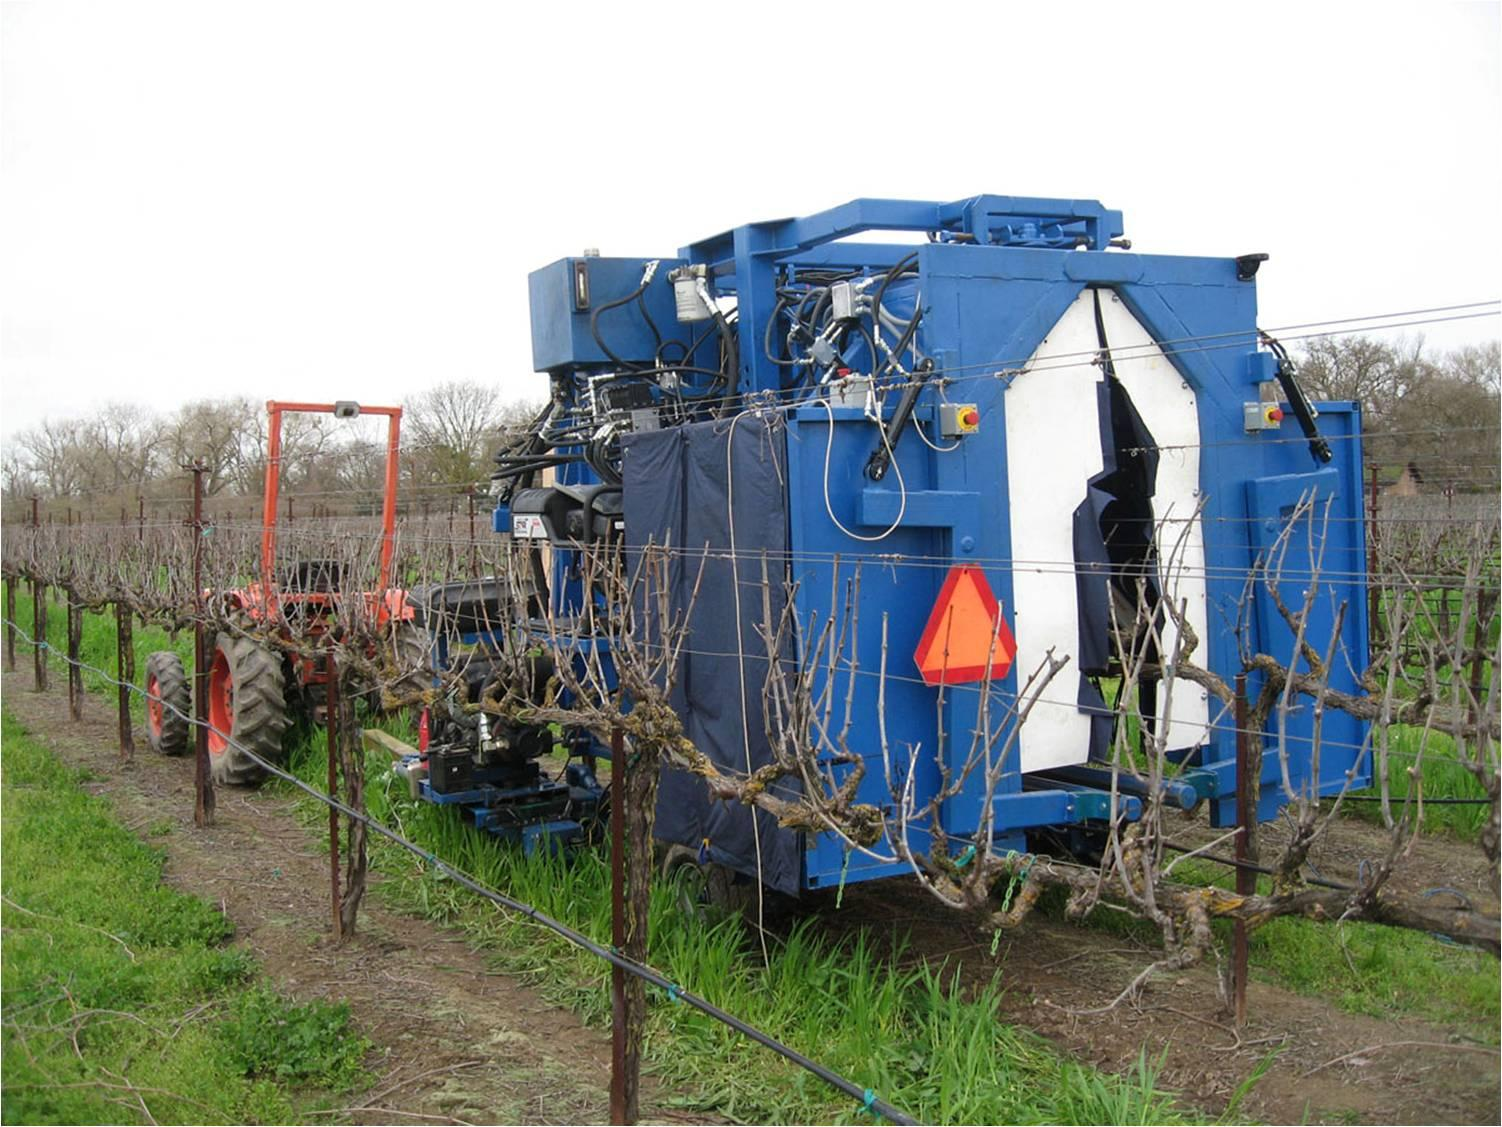
\includegraphics[width=.8\linewidth]{Images/blueTrain.jpg}
  \captionof{figure}{blue train}
\end{minipage}%
\begin{minipage}{.5\textwidth}
  \centering
  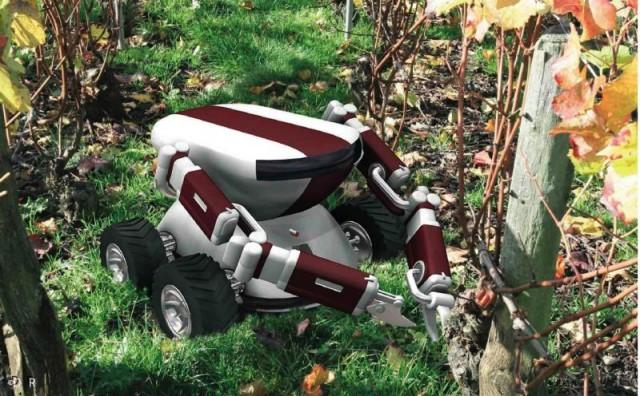
\includegraphics[width=.8\linewidth]{Images/brownrobot.jpg}
  \captionof{figure}{brown robot}
\end{minipage}
\end{figure}
However, as previously stated, the simple task of picking produce is very complicated. In general, an automated system must be able to first distinguish that the produce exists amongst other real-world objects, then go through a series of motions and information transactions in order to retrieve the produce safely, then navigate its sensors to the next possible location of produce to start the process over again.
\myfigure{Images/greenTracktor.jpg}{Robotic Strawberry Harvester by Robotic Harvesting, LLC}{.5}
With this in mind, the goal of this research is to produce a system by which an autonomous robot can, after detection of its target, maneuver a robotic arm through obstacles to capture and retrieve the detected produce. When used in concert with the work from our Perception and Mapping team developments through the robot produced by our Modification team, our target will be a green bell pepper, but it is planned that the robot will be able to function with other produce targets and will be able to be tailored to other robots of similar construction. The boon this will offer to the agricultural industry is obvious, as it greatly reduces the cost to only the initial price of the robot, power, and the manpower necessary to provide maintenance for the machine, which may be left to warranty or the owner.
\section{Goals}
When completed, the program will be able to process location data from a world map for navigation, know when a target has been perceived, guide the picking arm to its target in real time, and plot and execute a route to the location of a potential target. These tasks will be broken up as follows:
\begin{enumerate}
\item Robot path finding
\begin{enumerate}
\item Process World Mapping
\item Steer and Drive
\end{enumerate}
\item Target detection
\begin{enumerate}
\item Process Perception
\end{enumerate}
\item Target retrieval
\begin{enumerate}
\item Instruct Robot Arm
\end{enumerate}
\end{enumerate}
In the long term, it is planned that the program will be able to operate for a variety of similar produce types with no changes other than the target to be detected, but will be easily alterable if alternative hardware is required for the produce retrieval. The end result will be the navigation to a bell pepper plant, the detection of a ripe fruit, and the harvesting of that fruit without damage.
In addition to this, we will also be implementing an easily extensible planning library that will be usable for several applications. The idea is that through our program you will be able to run many different planning programs that are not necessarily limited to that of a robot arm. The point of this generality is to make it easy to adapt our algorithms to other similar tasks.
\section{Background}
Previous semesters have been working on implementing various planing and controls algorithms. These implementations, however, have been independent efforts that must be integrated to ensure our goals are accomplished. Although solving the controls problem and the planning problem may be serious challenges in and of themselves, we cannot underestimate the importance of integration.

Primarily, what we have to work from is experience. We have several team-members that have gone through the work of implementing several algorithms and solving many of the problems independently. Their efforts served as proof-of-concept projects that show the basic functionality of what we are trying to accomplish with that particular module.

Unfortunately it is also true that their work was not necessarily implemented with the ideal of integration in mind. This means that although they know how to implement the system and did so very well as a stand-alone application, there are nuances that must be taken into account from the very design of the solution to ensure that it will be compatible with external systems. Indeed, we have implementations for controls algorithms, Rapidly-Randomly Exploring Trees, A* and point-cloud processing. This means we may have a large amount of code that may be copied or adapted from previous semesters. Still, because they did not have the idea of a planning and controls application at the moment of design, we will inevitably have to rework part of their solutions. Most-likely though we are going to use their work mainly to revise our own reworked implementation.
\section{Details}
\subsection{Software Design}
It is important to remember that many of the problems we are trying to solve with this application have been solved in previous semesters independently. Our challenge this iteration of the class is not to reinvent the wheel but rather to put its pieces together. To create an application that puts together all the solutions that we have worked on previously and make it into a flexible piece of software. 
Needless to say, developing and designing such a piece of software is non-trivial. In fact, we will probably spend most of our time dealing with the challenges that the software puts before us due to the complexity of the program rather than implementing the algorithms themselves. 
\subsubsection{Architecture}
Let us now begin with a rough idea of what our program will look like and how it will interact with the system in question: the robot.

As you can see in this image, our inputs will be the decoded sensorial information. Our application will be designed to be constantly receiving a stream of information that may be update at the leisure of the sensorial team. We will have an optimized data structure probably based on a multi-dimensional vector from libeigen or some other data-structure that we find more convenient. 
In the case that we face a data-structure so large that we are forced to deal directly with their structure, we will take precautions to ensure that such a case is not a problem. The main problem we are facing is how to deal with such a large number of unknowns in the code. We don't know exactly the data-structures or the information we will be receiving. To make our application flexible, we will have to keep it as abstract as possible maintaining interfaces and abstract classes that shield-us from any changes in the implementation of external components or even our own classes. Thus, the boxes you are seeing in that general application diagram are not the actual classes that will be doing the work but rather the interfaces that will interact with each other in a consistent way to ensure our complex system does not break in an even more complex way.
The next Diagram would be a more concrete implementation of our program in UML. Interfaces in this case would be the implementation equivalent of virtual classes. Notice though, that even with this more detailed diagram we still fail to capture the entirety of the problem at hand. There are plenty of additional problems and classes that need to be specified as we approach lower levels of implementation. These, however will accurately reflect the general modules of our program.
\myfigure{Images/SoftwareDesign/OverallApplication.jpg}{This is a UML representation of all our application. Only the interfaces are specified because everything will derive the same function signatures from them. The implementation of those functions though will be radically different depending on the situation.}{1}
We will be basing our application on the Model-View-Controller design pattern. The point of this pattern is to separate key components of the program to reduce decencies between components. This, in turn, increases the flexibility of the program and allows us to deal better with changes that we may have to implement later on. The idea is that the algorithms are, indeed, the logic of the program. These will process the input of the information and output useful information that is derived from those inputs. Algorithms is a common interface for any number of algorithms that we choose to implement to solve a planning problem. The PDataStructure class is simply a data-structure interface to allow the use for global data-structures across different algorithms. This is particularly useful for RRT's since the underlying data-structure will significantly impact the performance of our algorithm. Usually, we implement RRT's with k-d Trees. which is briefly mentioned since we must make the decision of either implementing it ourselves or adapting it from another library. The point of implementing data-structures with an interface is to experiment using different data-structures on the same algorithm.
\myfigure{Images/SoftwareDesign/500px-MVC-Process.png}{This is a rough schematic of what a model-view-controller system}{.4}
Thus, the controller or algorithms will handle everything logical that the application has to deal with. In our case, the User Interface or presenter, will be divided into two components. Since the user may need to pass information directly on the model(specially for testing purposes) we will allow the passing of certain information from Input to Space. In addition to this, the user must select which algorithm it wishes to run on the data given. This means that the user must also give commands to the control to ensure that the application carries out its task. The User Input class serves as an interface between the user and the rest of the application.
The other part of the view, is the Display or the part that deals with the visual outputs of our program. We must be able to represent visually at least some of the information that is given to us as a 2D map. This means that we will be showing not just the map given to us in terms of obstacles, goals and current position but we must also show the final paths but also the area explored by the algorithms. Notice, the decisions on how to represent all the information our application will have to handle is non-trivial and will require serious study.
Finally, we have the model: the container of all information. Our Space class serves as the model for our application since it will contain all information regarding the position of the robot. Notice, we will need to have more than one instance of Space in order to manage all the information efficiently. A joint-space will be required to handle the arm and a search of the join-space. A 3-D map of the area that is collected with our cameras will also be necessary to determine where the Joint Space maps into the 3D world we must interact with. Finally, we need 2D space that will give us information regarding the placement of the robot in the translational sense.
Remember though, the Point and Path interfaces serve as a way for Interfaces to exchange data regardless of the form in which it may be. This is simply the messengers that carry the information and are not part of the Model-View-Controller model.
The idea investing so much time in the design of our application is to ensure that we have a streamlined development and that the result is a maintainable application that future teams can build upon.

\subsubsection{Threading}
Probably the most difficult part in the implementation of this application will be handling the parallel processes that will be generated by the operation of the robot. This section is only an overview of what we will be having to be implementing. We will start our process with the source of our model: the vision sensors. These run on their own thread and will collect data independently of how fast we are running the algorithms. The job of space is to be updated constantly but only when an algorithm is not making use of the data-structure. We must check constantly whether there is updated data from the sensors and queue it for update with the latest version.
The algorithms will be running on their own thread that will begin execution with the detection of new sensory data. The algorithm will return a path or failure and either run again on automatic mode or await input from the user if we are simply trying to test the system. The data will then be stored in a path that is passed onto the controller.
The controller in turn also run on an independent thread that works at the speed at which the motors can execute the commands we give the robot. We must ensure that the data the controls are executing is the most up-to date information. Therefore, the path that the controls team executes must always be updating itself with the output of the algorithms. However, since we deal with the arm and the wheels separately, we have to ensure that we do not delay planning on the translation due to planning on the arm. This means that we will need to have at least two set of  space-algorithm-control threads. Ultimately, the idea of this section was to give an understanding of the complexity of the system we will be dealing with. 
\subsubsection{User Interface}
The Application we proposed will be a full functioned software. It is contained a powerful back end system architecture and a great front end GUI to interact with user.  Designed GUI of this application is shown below.
\myfigure{Images/SoftwareDesign/GUISample.jpg}{This is a simple portrayal of what the user interface will look  like}{1}
In this application, we will performance three major functions.
\begin{enumerate}
\item \textbf{Map and Path display:} Agricultural field map is being converted into a vector-image based 2-D map which will contain as much information about the filed as possible, After user choose a path search algorithm from algorithms selection area, and computing a passable path for robotics, the path will display on the map with blue line. 
\item \textbf{Real-time synchronization:}Robot will be placed in the display map with its current location in the field. It’s location will be updated in the display map. It will highlight the on-going paths the robot is taking and the places that the robot already visited in the previous attempt with a red line. When the simulation is running, it is updating the robot traveled path and feeding world map.
\item \textbf{Control Panel:}A dedicated control panel with a list tasks the robot can perform. In this display area, it is streaming the command performed by the robotics from corresponding API. However, at the back-end this application will translate the current position and preview position data, and callback the Youbot API to generate a valid control command for robot.
\end{enumerate}
\subsection{Controller Design}
Each joint of the Youbot has its motor controller. Specifically, each motor controller contains an ARM Cortex-M3 microcontroller, Hall Sensors, EtherCAT interfaces, and PID-Controllers. The PID-Controllers are further separated into position, velocity, and current PID-Controllers. Also, each joint has an I2t monitor that determines the square of the sum of the motor current over a period of time for safety measures. The control parameters have already been optimized and allows for relatively faster response time compared to the more common PI-Controllers. For simplicity, the group will begin by exploring the position controller and its related Youbot APIs.
\myfigure{Images/PositionController.png}{Position Controller in which the n stands for motor positions, e for errors, and other variables are optimized parameters.}{1}
\subsection{Youbot API}
The Youbot API consists of C++ open source libraries not only provides access to full firmware functionality, but also support joint level control. From commanding and sensing joint values including position, velocity, and current to manually tuning each joint parameter, the Youbot API provides a simple and direct method for implementing and testing mentioned planning algorithms. While the Youbot API supports base movement in the Cartesian space, the manipulator movement within the Cartesian space is not supported. Furthermore, the API does not provide any forward or inverse kinematics functionalities. From previous semester’s research, a possible inverse kinematic solution is the OpenRave IKFast library.   As part of the ROS framework, the IKFast conveniently outputs the necessary parameters Youbot joint command-calls require through numerical solving techniques.

Another important aspect of the Youbot API is that it encapsulates EtherCAT communication. Along with the EthercatMaster, the API provides a method of communication between the user application and the Youbot. Running an API with communication thread usually has a default cycle time of 1ms while running the API without a constant communication thread requires manual calls to methods such as sendProcessData() and receiveProcessData() scheduled by a real-time operating system (RTOS).
\myfigure{Images/youbotDriverOverview.png}{Diagram describing the communication threads and interactions within Youbot and between Youbot and user applications.}{.5}
\subsection{Path-Planning Algorithms}
\subsubsection{Graph Traversal Algorithms}
Finding the best shortest path in a workspace for a robot can be both challenging and frustrating. There are many processes that go into account concerning motion planning for the robot. Encompassing many applications, autonomy is the important key for our project as our goal is to create an autonomous robotic system. Motion planning algorithms are thus crucial in order to produce a continuous motion while avoiding collisions. One of the algorithms we will be considering is A* which is one of the most popular choices for pathfinding due to its flexibility. A* uses a best-first search, which is a search algorithm that navigates a graph of one or more goal points, or nodes. Like other graph-searching algorithms, in which it is capable of searching a huge area, one of the first steps before the beginning of the A* algorithm would be to simplify the search area before finding the path. At the starting point, a search is conducted taking into account the nodes around. Once the surrounding area is taken into account, the starting point is designated as a point of no interest or a closed node since the next step would be to take the first step on the path to the ending goal.
\myfigure{Images/planningProblem.png}{A model of the search area.}{.5}
Which direction to take is the question that is taken into consideration as the algorithm ranks the points surrounding the starting point on a certain basis. This basis is determined by two parameters, with one determining if the vertices are closer or farther than the starting point relative to the ending point and the other incorporating the use of heuristics. By using heuristics, an estimated distance from the remaining path can be calculated, which will help us develop the shortest path possible. Using these two parameters repeatedly will eventually form a path of possible points to take, and when taking into account any obstacles, the path will begin to unveil itself. These ranks the parameters establish can be modeled by a function, f(n) = g(n) + h(n) where g(n) reveals a cost to move from the starting point to a given node and h(n) reveals the heuristic. The steps to the path are used by the approach of maintaining an open nodes and closed nodes list. By keeping track of whether A* has already visited a node, A* will continue searching until the ending point has been reached or if for some reason the open nodes list is empty in which case there is no path.
\myfigure{Images/planningSolution.png}{A\* revealing the path to the goal}{.5}
While A* is widely used, there are other algorithms to take into account as well. D* is another approach in searching and pathfinding. In contrast to A*, D* begins searching by working backwards from the goal point. By producing a path based on given and assumed data, a path can be created while it is progressively updated due to any new information given about its surrounding area. This process is repeated until the destination coordinates are reached or if it’s been determined that there is no possible path. Similar to A*, D* maintains a list of nodes that are marked by a certain condition to be analyzed. RAISE and LOWER are two states specific to D* in which they reveal the cost of a node to be either higher or lower than the previous cost. Before a cost can be increased, the algorithm will check the neighboring nodes and observe if a deduction cost can be taken. If it is not possible, the RAISE state will spread among the nodes that contain backpointers which aid in developing the path. A backpointer denotes the next node directing to the target. The path will eventually be unveiled by following the backpointers. D* proves to be an efficient search algorithm while A* provides the shortest, lowest cost path, therefore it will be interesting to see which algorithm will work the best for our project.
\myfigure{Images/DStarMap.png}{A map revealing a path created by D\*}{.5}
\subsubsection{Random-Sampling Algorithms}
Previously, we have dealt with algorithms ideal for the relatively simple problem of 2D planning. These graph-search algorithms will promise completion and optimality when implemented correctly. Unfortunately, in order to achieve these promises we are going to have to pay the cost of a larger time complexity. In the 2D case we can handle with this time complexity simply because the data set can be handled effectively. However, when we are dealing with higher dimensions, (as is necessary when planning for a 5 degree of freedom robotic arm) we must utilize other algorithms that can find a solution in a reasonable amount of time. This family of algorithms does not promise completion or optimality. However, their ability to quickly explore such high-dimensional spaces, gives them a unique advantage when it comes to path-planning.
\paragraph{Rapidly-Randomly Exploring Trees}
The very most basic of these sample-based planning algorithms is the Rapidly Randomly Exploring Trees Algorithm. The most important points of this algorithms is that it is not able to promise us neither optimality(finding the best path) or completeness(finding a path if it exists). Another feature of this algorithm is that as we can see in the figures, the paths it creates are very erratic and far from a smooth trajectory we would like to see.Still, we can easily solve this problem with some path trimming. This process is simply taking points A and B which are connected through C and try to make a straight line between the two. We do this by checking if any point in the straight line has an obstacle. If it doesn't we simply remove point C and claim A and B to be connected with a straight line. The way our data structure will work, it is assumed that all points are connected by a straight line which means we would simply be removing C from the data structure.
The main feature of this algorithm is that it can relatively quickly find a viable path from which we can work on. Given the fact that we will be using threading in our application, it is essential to remember that we will have to use the most efficient algorithm to ensure that our path is relevant to the visual data we have.
The following is a rundown of the algorithm that is the core of all RRT's:
\begin{algorithm}
\caption{: BuildRRT}\\
Input: Initial configuration $q_{init}$, number of vertices in the RRT K, incremental distance $\Delta q$\\
Output: RRT graph $G$
\begin{algorithmic}[1]
\Function{G.init}{$q_{init}$}
\For{$k = 1$ \textbf{to} $K$}
\State $q_{rand} \gets \Call{RAND\_CONF}{}$
\State $q_{near} \gets \Call{NEAREST\_VERTEX}{q_{rand}, G}$
\State $q_{new} \gets \Call{NEW\_CONF}{q_{near}, q_{rand}, \Delta q}$
\State $G.\Call{add\_vertex}{q_{new}}$
\State$G.\Call{add\_edge}{q_{near}, q_{new}}$
\EndFor
\State \Return $G$
\EndFunction
\end{algorithmic}
\end{algorithm}

The process of building the RRT is rather simple. We need the initial position or $q_{init}$. We begin by adding this point to the tree. After that, we generate a random configuration in the space. It is important to note that we may constraint the search space so that only valid outputs are produced here. After that, we find the configuration in our tree that has the closest distance to the random point that is $q_{near}$. Still, we cannot add the random point for it could be a very long distance from even the nearest point in the tree. Thus we find the $q_{new}$ which is the a point a distance $\delta q$ from the $q_{near}$ in the direction of $q_{rand}$. That is finally the point that we add to the tree. The extension of this algorithm into a full planning algorithm is simply the addition of a stop condition when the goal is added to the tree.
Specifically for our purposes, all we are interested in doing is re-implementing RRT's with usability, extensibility and generality in mind. Ultimately, though, a simple RRT is only the beginning of what we intend to do with this application.
\paragraph{Bidirectional RRT's}
Soon after RRT's were discovered, we realized there was a way that could solve such hard multi-dimensional problems with ease. This method was simply adding another tree at the goal of our planning problem. These though, would be biased to select the nearest points in the other after a certain number of random selections. The result would be the generation of two large exploring trees that would grow towards each other. The algorithm is very similar to that of the original RRT's except it updates two trees.
\begin{algorithm}[H]
\caption{: Bidirectional Build RRT}
\begin{algorithmic}
\Function{RDT\_BALANCED\_BIDIRECTIONAL}{$q_{I},q_{G}$}
\For{$i=1 \textbf{to} K$}
\State $q_{n}$ \gets \Call{NEAREST}{$S_{a}, \alpha(i)$}
\State $q_{s}$ \gets \Call{STOPPING-CONFIGURATION}{$q_{n}, \alpha(i)$}
\If{$q_{s} \neq q_{n}$}
\State \Call{$T_{a}.add\_vertex$}{$q_{s}$}
\State \Call{$T_{a}.add\_edge$}{$q_{n}, q_{s}$}
\State $q_{n}'$ \gets \Call{NEAREST}{$S_{b}, q_{s}$}
\State $q_{s}'$ \gets \Call{STOPPING-CONFIGURATION}{$q_{n}', q_{s}$}
\If{$q'_{s} \neq q_{n}'$}
\State \Call{$T_{b}.add\_vertex$}{$q_{s}'$}
\State \Call{$T_{b}.add\_edge$}{$q'_{n},q_{s}'$}
\If{$q_{s}' = q_{s}$}
\State \Return SOLUTION
\EndIf
\If{$|T_{b}|>|T_{a}|$}
\State \Call{SWAP}{$T_{a},T_{b}$}
\EndIf
\EndIf
\EndIf
\EndFor
\State \Return FAILURE
\EndFunction
\end{algorithmic}
\end{algorithm}
As you can see, all we are doing is growing two RRT's and making sure that they are balanced. This means that no tree is larger and the other. It is important to take into account that sometimes we switch the tree at $T_{a}$ with the tree at $T_{b}$. Still this is not much different than doubly implementing the previous algorithm with a slight twist. Despite the simplicity though, the improvements in speed are significant.
\paragraph{RRT*}
RRT* holds the same principles as the original RRT's. You are using random sampling to generate a path. That however, is where the similarities end. This Algorithm utilizes the dynamic programming to ``rewire'' the tree whenever it receives information from a new random point.  This means that this new version means that it is asymptotic optimal. This means that the longer you run the algorithm the more it will approach optimality. this might be useful if we have condition that allow us extra computing time between time-steps. This, however, comes at a cost. The algorithm maintains additional information from what is usually kept in a simple RRT. Although we incur a heavy memory cost, this optimality could be extremely could prove useful.
\myfigure{Images/SamplePlanning/RRTStarAlgorithm.png}{This is an overview of the implementation of RRT*. Although it uses an RRT, it constantly updates it an adds new paths between the points in search of an optimal configuration with-in the sampled space.}{1}
Despite the advantages of the algorithm, we must remember that an there is also an intrinsic difficulty in the complexity of implementing the algorithm. In this case, we are dealing with five different sub-algorithms that coalesce into the results we see. 
\myfigure{Images/SamplePlanning/AlgorithmComparison.png}{As you can see, the asymptotic behavior of the different algorithms varies wildly between each implementation of RRT. This behavior is very important given the large amount of data we will probably have to process.}{1}
\paragraph{RRT\#}
Finally, RRT\# is our ultimate end-game for RRT's. Having been recently developed this is an even more advanced rework of RRT*. The idea behind RRT\# is that we can improve our memory usage and speed by only keeping points that are locally relevant to our area of search and that therefore have a possibility of being optimal. Unfortunately, once again, the problem arises from the sheer complexity of implementing this algorithm. Since we would have basic planning functionality for the arm with only implementing basic RRT's it is worth considering implementing this algorithm as a challenge that may add to the functionality of our program but will do nothing more than optimize an existing basic functionality.
%\myfigure{Images/SamplePlanning/rrtvsrrtstar2.jpg}{As you can see RRT\# has a fundamentally different behavior from RRT* which is designed to use less computational resources. You can see RRT* on the top and RRT\# on the bottom. Each on an increasing number of steps.}{1}
\section{Collaboration}
Since the team’s responsibilities span from planning the robots route to implementing and controlling the robot’s movement, it is easier for other sub-teams to picture this team’s pipeline as a “black box”. Information transfer and implementation within the team will be independent from the processes of the other sub-teams. The idea is to create an application with the necessary APIs to communicate with other teams while dealing with inputs from other teams within our application. Specifics of the interfaces between other sub-teams will have to be discussed during the beginning phases of the project. It is crucial for each sub-team to recognize required inputs and possible output formats. For example, in order to generate the best route using mapping team’s data, the planning team will have to be able to process the output data for the map. Will the agreed format be .vtk generated from navigation meshes (the mapping algorithm from previous semester) or will the mapping team decide to explore other possible mapping algorithms? Questions like these will have to answer through cross-team discussion in order to successfully implement the interface.

Information from the mapping team will be utilized to generate the most efficient route possible. The team expects some sort of map data communicated through agreed APIs and will utilize the data to generate the route through its own thread processes. After receiving the needed poses, the control team will be responsible of moving the robot and this will provide the perception team with the updated coordinates of the robot without any explicit output from the controls team.   

Aside from weekly meetings that will allow each team to update their progresses, urgent questions regarding implementation details can be posted and answered utilizing the team’s forum. With each team member capable of posting questions, answers, and follow-ups, confusion about other team’s work can be minimized. Furthermore, blog posts regarding each individual’s work on his/her research will also allow teammates to understand the technology and research utilized during the progression of the project.
\section{Conclusion}
In conclusion we are not only implementing algorithms or processing mapping data. This project is not simply about having theoretical results for a stand-alone program. Our focus this time will be on the difficulty of software engineering. We are going to have to integrate several very complex systems into a streamlined application that can elegantly deal with the problem at hand. To successfully execute this, we will need to ensure the flexibility of our code through heavy abstraction and placing interfaces between key components of our program. At this time we have been tasked with the over-all integration of the systems that have been designed previously and are being done this semester. 

Our problem is not difficult due to the nature but rather the complexity of our problem. Although there are way to minimize the detrimental effects this can have on the development of a system, there is no question our task remains daunting. However, should we succeed, we would have generated a working application that will be not only useful for this planning particular planning problem but for any other problem of a similar nature that may come after. Our vision is that of a flexible application that with relatively little implementation can adapt implemented algorithms into different but similar planning problems. Few things are worth the time invested more than a flexible library that can be used in a multitude of problems.
\newpage
\begin{thebibliography}{20}
\bibitem{VisionRobotics} \href{http://visionrobotics.com/vrc/index.php?option=com_zoom&Itemid=26&catid=6}{Vision Robotics}
\bibitem{wallye} \href{http://wall-ye.com/}{Wall-Ye}
\bibitem{roboticcharvest} \href{http://www.roboticharvesting.com/products.html}{Robotic Harvesting}
\bibitem{kuka} \href{http://www.kuka-labs.com/en/service_robotics/research_education/youbot/}{Kuka Labs}
\bibitem{robocup} \href{http://www.robocupatwork.org/download/RoboCup-At-Work_Camp_2012/RAW_Camp2012-Jan-Paulus_youBotAPI.pdf}{RoboCup}
\bibitem{metu} \href{http://www.eee.metu.edu.tr/~ee402/2013/EE402RecitationReport_4.pdf}{Metu}
\bibitem{Astar} \href{http://en.wikipedia.org/wiki/A*_search_algorithm}{A*}
\bibitem{AstarTutorial} \href{http://www.policyalmanac.org/games/aStarTutorial.htm}{A* Tutorial}
\bibitem{AstarCompare} \href{http://theory.stanford.edu/~amitp/GameProgramming/AStarComparison.html}{A* Comparison}
\bibitem{heuristics} \href{http://www.policyalmanac.org/games/heuristics.htm}{Heuristics}
\bibitem{dynamicp} \href{http://www.frc.ri.cmu.edu/~axs/dynamic_plan.html}{Dynamic Planning}
\bibitem{dstar} \href{http://en.wikipedia.org/wiki/D*}{D*}
\bibitem{RRT} \href{http://msl.cs.uiuc.edu/rrt/papers.html}{Rapidly-Exploring Random Trees}
\bibitem{RRTBidi} \href{http://people.csail.mit.edu/aperez/obirrt/}{Bidirectional RRTs}
\bibitem{RRTstar} \href{http://sertac.scripts.mit.edu/web/?page_id=15}{RRT*}
\bibitem{RRTsharp} \href{http://ieeexplore.ieee.org/xpl/login.jsp?tp=&arnumber=6630906&url=http://ieeexplore.ieee.org/iel7/6615630/6630547/06630906.pdf?arnumber=6630906}{RRT\#}
\bibitem{kdtree} \href{https://www.cise.ufl.edu/class/cot5520fa09/CG_RangeKDtrees.pdf}{K-D Trees}
\end{thebibliography}

\end{document}
